\documentclass[tikz,dvipdfmx,dvipsnames]{standalone}

\usepackage{amsmath, amssymb, amsthm, mathrsfs, amsfonts, dsfont}
\usepackage{bbm}
\usepackage{bm}
\usepackage{physics}
\usepackage{ifthen}
\usepackage{setspace}
\usepackage{mathtools}
\usepackage{svg}

\newcommand{\defeq}{\coloneqq}

\newcommand{\red}[1]{\textcolor{red}{#1}}
\newcommand{\blue}[1]{\textcolor{blue}{#1}}
\newcommand{\cyan}[1]{\textcolor{cyan}{#1}}
\newcommand{\gray}[1]{\textcolor{gray}{#1}}
\newcommand{\green}[1]{\textcolor{green}{#1}}
\newcommand{\brown}[1]{\textcolor{brown}{#1}}
\newcommand{\black}[1]{\textcolor{black}{#1}}
\newcommand{\orange}[1]{\textcolor{orange}{#1}}
\newcommand{\purple}[1]{\textcolor{purple}{#1}}
\newcommand{\yellow}[1]{\textcolor{yellow}{#1}}
\newcommand{\Magenta}[1]{\textcolor{Magenta}{#1}}
\newcommand{\RoyalBlue}[1]{\textcolor{RoyalBlue}{#1}}
\newcommand{\RubineRed}[1]{\textcolor{RubineRed}{#1}}
\newcommand{\ForestGreen}[1]{\textcolor{ForestGreen}{#1}}
\newcommand{\YellowOrange}[1]{\textcolor{YellowOrange}{#1}}
\newcommand{\WildStrawberry}[1]{\textcolor{WildStrawberry}{#1}}

\usetikzlibrary{calc,matrix,math}
\usetikzlibrary{decorations.pathreplacing,calligraphy,shapes.arrows}

\usetikzlibrary{
  3d,
  calc,
  math,
  matrix,
  patterns,
  backgrounds,
  arrows.meta,
  shapes.geometric
}


\definecolor{c0}{RGB}{253, 231, 36}
\definecolor{c1}{RGB}{154, 216, 60}
\definecolor{c2}{RGB}{91, 200, 98}
\definecolor{c3}{RGB}{59, 81, 138}
\definecolor{c4}{RGB}{69, 50, 127}

\definecolor{cA}{HTML}{0072BD}
\definecolor{cB}{HTML}{EDB120}
\definecolor{cC}{HTML}{77AC30}
\definecolor{cD}{HTML}{D95319}

\begin{document}

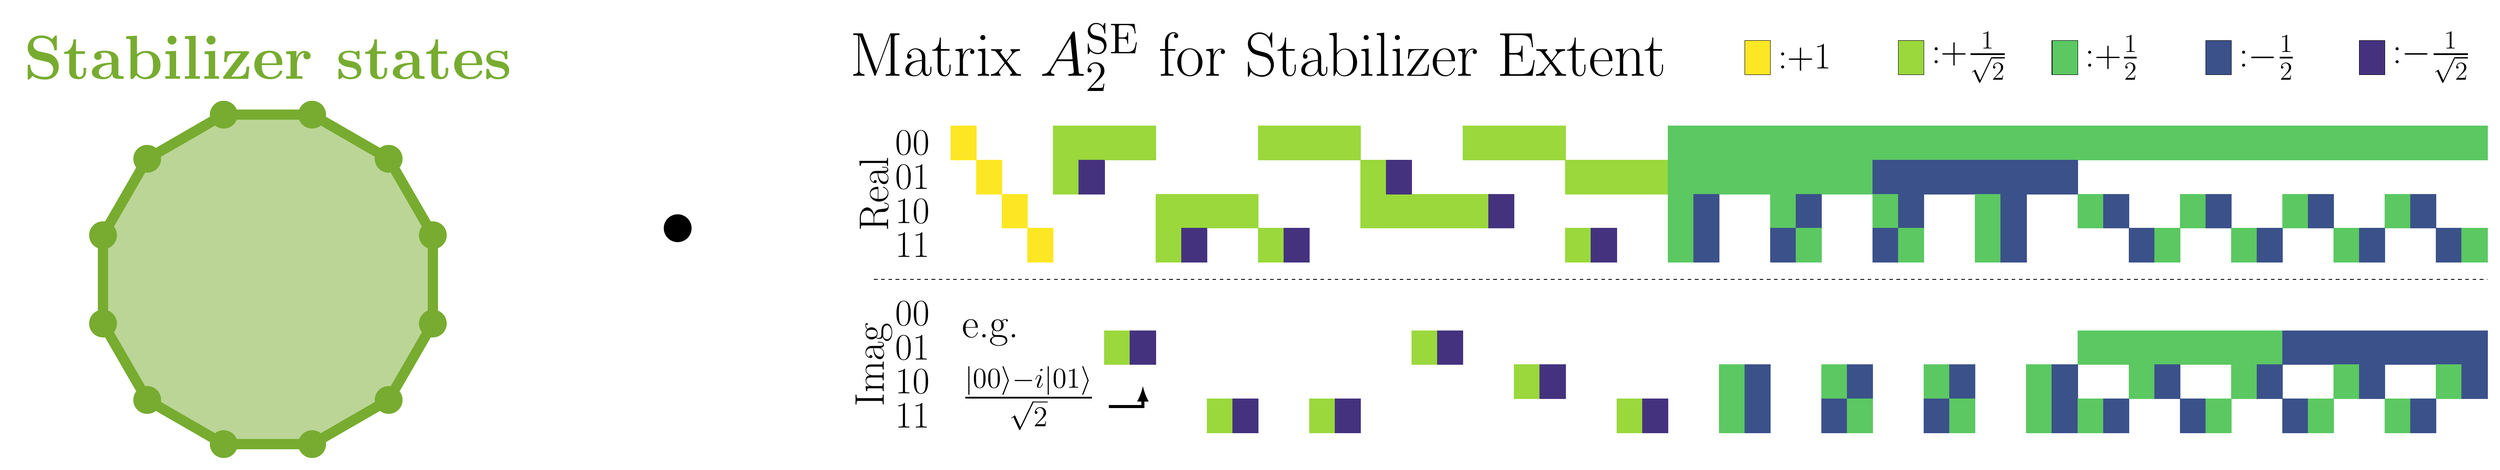
\begin{tikzpicture}[xscale=0.75]
    \begin{scope}
        \foreach \color/\col/\row in {
                c0/0/0,
                c0/1/-1,
                c0/2/-2,
                c0/3/-3,
                c1/4/0,
                c1/4/-1,
                c1/5/0,
                c4/5/-1,
                c1/6/0,
                c1/6/-6,
                c1/7/0,
                c4/7/-6,
                c1/8/-2,
                c1/8/-3,
                c1/9/-2,
                c4/9/-3,
                c1/10/-2,
                c1/10/-8,
                c1/11/-2,
                c4/11/-8,
                c1/12/0,
                c1/12/-3,
                c1/13/0,
                c4/13/-3,
                c1/14/0,
                c1/14/-8,
                c1/15/0,
                c4/15/-8,
                c1/16/-2,
                c1/16/-1,
                c1/17/-2,
                c4/17/-1,
                c1/18/-2,
                c1/18/-6,
                c1/19/-2,
                c4/19/-6,
                c1/20/0,
                c1/20/-2,
                c1/21/0,
                c4/21/-2,
                c1/22/0,
                c1/22/-7,
                c1/23/0,
                c4/23/-7,
                c1/24/-1,
                c1/24/-3,
                c1/25/-1,
                c4/25/-3,
                c1/26/-1,
                c1/26/-8,
                c1/27/-1,
                c4/27/-8,
                c2/28/0,
                c2/28/-1,
                c2/28/-2,
                c2/28/-3,
                c2/29/0,
                c2/29/-1,
                c3/29/-2,
                c3/29/-3,
                c2/30/0,
                c2/30/-1,
                c2/30/-7,
                c2/30/-8,
                c2/31/0,
                c2/31/-1,
                c3/31/-7,
                c3/31/-8,
                c2/32/0,
                c2/32/-1,
                c2/32/-2,
                c3/32/-3,
                c2/33/0,
                c2/33/-1,
                c3/33/-2,
                c2/33/-3,
                c2/34/0,
                c2/34/-1,
                c2/34/-7,
                c3/34/-8,
                c2/35/0,
                c2/35/-1,
                c3/35/-7,
                c2/35/-8,
                c2/36/0,
                c3/36/-1,
                c2/36/-2,
                c3/36/-3,
                c2/37/0,
                c3/37/-1,
                c3/37/-2,
                c2/37/-3,
                c2/38/0,
                c3/38/-1,
                c2/38/-7,
                c3/38/-8,
                c2/39/0,
                c3/39/-1,
                c3/39/-7,
                c2/39/-8,
                c2/40/0,
                c3/40/-1,
                c2/40/-2,
                c2/40/-3,
                c2/41/0,
                c3/41/-1,
                c3/41/-2,
                c3/41/-3,
                c2/42/0,
                c3/42/-1,
                c2/42/-7,
                c2/42/-8,
                c2/43/0,
                c3/43/-1,
                c3/43/-7,
                c3/43/-8,
                c2/44/0,
                c2/44/-6,
                c2/44/-2,
                c2/44/-8,
                c2/45/0,
                c2/45/-6,
                c3/45/-2,
                c3/45/-8,
                c2/46/0,
                c2/46/-6,
                c2/46/-7,
                c3/46/-3,
                c2/47/0,
                c2/47/-6,
                c3/47/-7,
                c2/47/-3,
                c2/48/0,
                c2/48/-6,
                c2/48/-2,
                c3/48/-8,
                c2/49/0,
                c2/49/-6,
                c3/49/-2,
                c2/49/-8,
                c2/50/0,
                c2/50/-6,
                c2/50/-7,
                c2/50/-3,
                c2/51/0,
                c2/51/-6,
                c3/51/-7,
                c3/51/-3,
                c2/52/0,
                c3/52/-6,
                c2/52/-2,
                c3/52/-8,
                c2/53/0,
                c3/53/-6,
                c3/53/-2,
                c2/53/-8,
                c2/54/0,
                c3/54/-6,
                c2/54/-7,
                c2/54/-3,
                c2/55/0,
                c3/55/-6,
                c3/55/-7,
                c3/55/-3,
                c2/56/0,
                c3/56/-6,
                c2/56/-2,
                c2/56/-8,
                c2/57/0,
                c3/57/-6,
                c3/57/-2,
                c3/57/-8,
                c2/58/0,
                c3/58/-6,
                c2/58/-7,
                c3/58/-3,
                c2/59/0,
                c3/59/-6,
                c3/59/-7,
                c2/59/-3
            }{
                \draw[
                    fill=\color,
                    draw=\color
                ] (\col, \row) rectangle (\col + 1, \row - 1);
            }
    \end{scope}

    \begin{scope}
        \foreach \row/\label in {
                -0.5/00,
                -1.5/01,
                -2.5/10,
                -3.5/11,
                -5.5/00,
                -6.5/01,
                -7.5/10,
                -8.5/11
            }{
                \node[anchor=center,font=\LARGE,scale=1.8]
                at (-1.5, \row) {\label};
            }

        \node[anchor=center,font=\LARGE,rotate=90,scale=2]
        at (-3, -2) {Real};
        \node[anchor=center,font=\LARGE,rotate=90,scale=2]
        at (-3, -7) {Imag};

        \draw[dashed] (-3,-4.5) -- (60,-4.5);
    \end{scope}

    \node[font=\LARGE,scale=2,align=left] at (4,-7.3) {e.g.\\[1ex]$\frac{\ket{00}-i\ket{01}}{\sqrt{2}}$ \tikz{\draw[-latex,very thick] (-0.5,0) -| (0,0.3);}};
    \node[font=\LARGE,scale=3,align=left] at (12,+2) {Matrix $A_2^{\text{SE}}$ for Stabilizer Extent};
    \node[font=\LARGE,scale=3] at (-26.666,+2) {\color{cC}\textbf{Stabilizer states}};

    \begin{scope}
        \draw[fill=c0] (25+6*1, 2+0.5) rectangle (26+6*1, 2-0.5);
        \draw[fill=c1] (25+6*2, 2+0.5) rectangle (26+6*2, 2-0.5);
        \draw[fill=c2] (25+6*3, 2+0.5) rectangle (26+6*3, 2-0.5);
        \draw[fill=c3] (25+6*4, 2+0.5) rectangle (26+6*4, 2-0.5);
        \draw[fill=c4] (25+6*5, 2+0.5) rectangle (26+6*5, 2-0.5);
        \node[anchor=west,font=\LARGE,scale=1.8] at (26+6*1, +2) {:$+1$};
        \node[anchor=west,font=\LARGE,scale=1.8] at (26+6*2, +2) {:$+\frac{1}{\sqrt{2}}$};
        \node[anchor=west,font=\LARGE,scale=1.8] at (26+6*3, +2) {:$+\frac{1}{2}$};
        \node[anchor=west,font=\LARGE,scale=1.8] at (26+6*4, +2) {:$-\frac{1}{2}$};
        \node[anchor=west,font=\LARGE,scale=1.8] at (26+6*5, +2) {:$-\frac{1}{\sqrt{2}}$};
    \end{scope}

    \begin{scope}[xscale=1.333333333333,xshift=-20cm,yshift=-4.5cm]
        \node[regular polygon, regular polygon sides=12,minimum size=10cm,draw,line width=0.3cm,cC,fill=cC!50] (fs) at (0,0) {};
        \foreach \x in {1,...,12}
        \filldraw[cC] ({5*sin(15+30*\x)},{5*cos(15+30*\x)}) circle[radius=0.4cm];

        \coordinate (Rho) at (+12,+1.5);
        \filldraw (Rho) circle (0.4cm);
    \end{scope}

\end{tikzpicture}

\end{document}